\chapter{Trilateration-based reconstruction of  decays into photons}\label{chapter:gps}

Reconstruction of a point of a particle decay, commonly performed for charged particles using tracking devices such as drift chambers or solid state pixel detectors, becomes a much more challenging task in case of processes which only contain neutral states. The two cases discussed in this work, the \ops/$\to 3\gamma$ annihilation and the long-lived neutral K meson decay $\Kl\to 3\pi^0\to 6\gamma$, although occurring at vastly different energy scales and governed by different mechanisms, possess the same experimental difficulties when it comes to their reconstruction using only the resulting photons recorded by a detector. This Chapter presents a technique based on trilateration which allows for determination of the decay point and time for both of the aforementioned processes.

\section{Application of trilateration to reconstruction of particle decays}
\label{sec:general_trilateration}
Trilateration is well-established method of localizing points which are known to lie simultaneously on surfaces of several spheres or circles whose centers correspond to certain reference points. In the classical trilateration problem, both reference points and spheres' radii are well defined and knowledge of three non-identical and mutually intersecting spheres is sufficient to calculate the position of the sought common point. In fact, trilateration using three references can yield up to two solutions (in general, the intersection of two spheres is a circle which can have 0, 1 (in case of tangency) or 2 intersection points with a third sphere) and additional criteria must be applied to disambiguate the point being localized.

Practical applications of trilateration commonly measure the spheres' radii through the time of propagation of a certain signal between the localized point and the known references. This is the case in e.g. the Global Positioning System (GPS)~\cite{Langley2005TheMO, Carter1999PrinciplesOG} where references constituted by satellite locations exchange radio signals with the receiver whose position is sought. In such an approach, however, both the references and the localized object must measure the signal emission and recording time with respect to a single origin, which is often impossible. To resolve this issue, radii of the spheres must be parametrized with an additional unknown (besides the three spatial coordinates) being either the start or stop time of the exchanged signal. As the reconstruction problem with three references and variable spheres' radii is underdetermined, additional information must be included in the system, e.g.\ by using a fourth reference point. On the other hand, a useful consequence in this case is that the initially unknown time is obtained from the reconstruction as a by-product additional to the spatial coordinates, e.g.\ in the GPS system the localized receiver determines the current time precisely besides its position.

Such extended trilateration approach similar to GPS positioning has been adapted to reconstruction of neutral states into several photons. In this case, the place of decay is the localized object, final state photons serve as the exchanged signal whereas the recording points and times of their interactions in the detector provide the references. Details of the general reconstruction problem as well as its solution are discussed in the next Section on the example of $\Kl\to 3\pi^0\to 6\gamma$ decay while~\sref{sec:gps_jpet} presents a slightly different case of \ops/$\to 3\gamma$, where the decay point is obtained with three reference points only.

\section{Reconstruction of $\Kl\to 3\pi^0 \to 6 \gamma$ in KLOE}\label{sec:gps_kloe}
As discussed in Sections~\ref{sec:kaons} and~\ref{sec:kloe}, the lifetime of the $\Kl$ meson in the KLOE detector frame of reference is sufficiently large for the meson to decay anywhere in the detector volume. This fact calls for reconstruction procedures capable for localizing a $\Kl$ decay based on its products with comparable performance for any distance of the decay from the detector center. In case of decays involving charged products, this is catered for by the drift chamber filling almost the entire detector. In case of the $\Kl\to 3 \pi^0$ process%
\footnote{As the mean $\pi^0$ lifetime, $(8.52\pm0.18)\times 10^{-17}$~s, is unregisterably small for KLOE and the branching fraction for the $\pi^0\to\gamma\gamma$ decay is $98.823\pm0.034$~\%, further in this work the process $\Kl\to 3\pi^0\to 6\gamma$ will always be considered.}%
, the most prominent among all-neutral decays of the long-lived neutral K meson, multiple studies performed in KLOE have augmented its reconstruction with information coming from the decay of a second kaon ($\Ks$) originating from the same $\phi$ decay~\cite{difalco_phd,kloe_kl3pi0_br,kloe_kl_lifetime}. If the accompanying kaon decay is chosen e.g.~as $\Ks\to\pi^+\pi^-$ for which DC-based reconstruction of the two pion tracks yields a very precise determination of the $\Ks$ momentum vector, the kinematics of the $\phi\to\Ks\Kl$ decay along with known average $\phi$ boost provide an estimate of the $\Kl$ momentum direction as shown in~\sref{sec:ks_from_kl}. Consequently, the $\Kl\to 3 \pi^0\to 6 \gamma$ decay vertex can be found along the known $\Kl$ line of flight by considering the sum of times of flight of the kaon and and even a single photon~\cite{data_handling}. This approach, however, is not applicable in case of the \Ts~symmetry test described in~\cref{chapter:test_kloe} where the process under study is defined by final states of both kaon decays and $\Kl\to 3\pi^0$ must be accompanied by a semi-leptonic decay of $\Ks$ (see~\tref{tab:processes}). Then, the unregistered neutrino momentum prevents a good reconstruction of $\vec{p}_{\Ks}$ and thus also the $\Kl$ line of flight. To avoid these difficulties, the trilateration technique has been employed in the localization of the $\Kl\to 3\pi^0$ decay without relying on any information except up to 6 photons recorded in the electromagnetic calorimeter of KLOE.

\begin{figure}[h!]
  \centering
  % PIC 1
  \captionsetup[sub]{margin=1ex}
  \begin{subfigure}{0.45\textwidth}
    \begin{tikzpicture}[scale=0.45,photon/.style={->, ultra thick, black},]
    \coordinate (clu1) at (-4.58,2);
    \coordinate (clu2) at (1,4.90);
    \coordinate (clu3) at (4,3);
    \coordinate (clu4) at (4.90,-1);
    \coordinate (clu5) at (-2,4.58);
    \coordinate (clu6) at (4.90, 1.0);
    \coordinate (vertex) at (1.0,2.0);

    % draw a fake arc and text to keep the same size of the picture as the next ones
    \draw[thick, white, rotate=85, dashed] (clu1)+(-5.58,0) arc (180:320:5.58);
    \node[white,anchor=south] at (clu1) {\scriptsize$(\!X_1\!,\!Y_1\!,\!Z_1\!,\!T_1\!)$};
    
    \draw[gray, line width=4pt] (0,0) circle (5);
    \draw[red,fill] (clu1) circle (0.2);
    \draw[darkgreen,fill] (clu2) circle (0.2);
    \draw[blue,fill] (clu3) circle (0.2);
    \draw[orange,fill] (clu4) circle (0.2);
    \draw[yellow,fill] (clu5) circle (0.2);
    \draw[violet,fill] (clu6) circle (0.2);

    \draw[black,dashed,->] (0,0) -- (vertex) node[midway, right,yshift=-2mm] {\footnotesize $\Kl$};
    \draw[darkgray,fill] (0,0) circle (0.1) node[left]{$\phi$};
    \draw[darkgray,fill] (vertex) circle (0.1);
    
    \draw[snake it,->] (vertex) -- (clu1) node[midway, above]{$\gamma$};
    \draw[snake it,->] (vertex) -- (clu2) node[midway, left]{$\gamma$};
    \draw[snake it,->] (vertex) -- (clu3) node[midway, above]{$\gamma$};
    \draw[snake it,->] (vertex) -- (clu4) node[midway, above]{$\gamma$};
    \draw[snake it,->] (vertex) -- (clu5) node[midway, above]{$\gamma$};
    \draw[snake it,->] (vertex) -- (clu6) node[midway, above]{$\gamma$};
    
  \end{tikzpicture}
  \caption{Schematic presentation of a \mbox{$\Kl\to 3\pi^0\to 6 \gamma$} decay in the transverse view of KLOE EMC (gray band) which records at maximum 6 photon interaction points (labeled with dots of different colors).}\label{fig:trilateration_kloe_a}.
\end{subfigure}
% PIC 2
  \begin{subfigure}{0.45\textwidth}
  \begin{tikzpicture}[scale=0.45,photon/.style={->, ultra thick, black},]
    \coordinate (clu1) at (-4.58,2);
    \coordinate (clu2) at (1,4.90);
    \coordinate (clu3) at (4,3);
    \coordinate (clu4) at (4.90,-1);
    \coordinate (clu5) at (-2,4.58);
    \coordinate (clu6) at (4.90, 1.0);
    \coordinate (vertex) at (1.0,2.0);
    
    \draw[gray, line width=4pt] (0,0) circle (5);    \draw[red,fill] (clu1) circle (0.2);
    \draw[darkgreen,fill] (clu2) circle (0.2);
    \draw[blue,fill] (clu3) circle (0.2);
    \draw[orange,fill] (clu4) circle (0.2);
    \draw[yellow,fill] (clu5) circle (0.2);
    \draw[violet,fill] (clu6) circle (0.2);

    \node[black,anchor=south] at (clu1) {\scriptsize$(\!X_1\!,\!Y_1\!,\!Z_1\!,\!T_1\!)$};
    \draw[thick, red,rotate=85, dashed] (clu1)+(-5.58,0) arc (180:320:5.58);
    
    \draw[red,->] (0.63, 0) -- (-4.3,1.9) node[midway, above] {$\gamma$} node[midway, below, black,xshift=-3mm,yshift=-2mm] {\footnotesize $R^\gamma_1\!=\!c(T_1\!-\!t_d)$};
  \end{tikzpicture}
  \caption{For each of the points of $\gamma$ interaction in the detector, a set of possible creation points of this $\gamma$ quantum is a sphere (dashed line) centered at the known location of the EMC cluster and with a radius parametrized by an unknown time $t_d$ of $\Kl$~decay.}\label{fig:trilateration_kloe_b}
\end{subfigure}
  % PIC 3
  \begin{subfigure}{0.45\textwidth}
  \begin{tikzpicture}[scale=0.45,photon/.style={->, ultra thick, black},]
    \coordinate (clu1) at (-4.58,2);
    \coordinate (clu2) at (1,4.90);
    \coordinate (clu3) at (4,3);
    \coordinate (clu4) at (4.90,-1);
    \coordinate (clu5) at (-2,4.58);
    \coordinate (clu6) at (4.90, 1.0);
    \coordinate (vertex) at (1.0,2.0);

    % draw a fake text to keep the same size of the picture as the next ones
    \node[white,anchor=south] at (clu1) {\scriptsize$(\!X_1\!,\!Y_1\!,\!Z_1\!,\!T_1\!)$};
    
    \draw[gray, line width=4pt] (0,0) circle (5);
    \draw[red,fill] (clu1) circle (0.2);
    \draw[darkgreen,fill] (clu2) circle (0.2);
    \draw[blue,fill] (clu3) circle (0.2);
    \draw[orange,fill] (clu4) circle (0.2);
    \draw[yellow,fill] (clu5) circle (0.2);
    \draw[violet,fill] (clu6) circle (0.2);

    \draw[thick, red,rotate=85, dashed] (clu1)+(-5.58,0) arc (180:320:5.58);
    \draw[thick, darkgreen,rotate=-10,dashed] (clu2)+(-2.90,0) arc (180:360:2.90);
    \draw[thick, blue,rotate=-55,dashed] (clu3)+(-3.16,0) arc (180:360:3.16);
    \draw[thick, orange,rotate=-90, dashed] (clu4)+(-4.92,0) arc (180:330:4.92);

    % \draw[black,fill] (vertex) circle (0.15) node[below, yshift=1mm, xshift=-8mm]{\footnotesize $(x\!,y\!,z\!,t)$};
    \draw[black,fill] (vertex) circle (0.15) node[below, yshift=2mm, xshift=-11mm]{\footnotesize $(x_d,y_d,z_d,t_d)$};        
  \end{tikzpicture} 
  \caption{The $\Kl\to 3\pi^0 \to 6 \gamma$ decay vertex is found as an analytically-calculated intersection of the possible origin spheres of at least 4 recorded photons.}\label{fig:trilateration_kloe_c}
\end{subfigure}
% PIC 4
\begin{subfigure}{0.45\textwidth}
    \begin{tikzpicture}[scale=0.45,photon/.style={->, ultra thick, black},]
    \coordinate (clu1) at (-4.58,2);
    \coordinate (clu2) at (1,4.90);
    \coordinate (clu3) at (4,3);
    \coordinate (clu4) at (4.90,-1);
    \coordinate (clu5) at (-2,4.58);
    \coordinate (clu6) at (4.90, 1.0);
    \coordinate (vertex) at (1.0,2.0);

    % draw a fake text to keep the same size of the picture as the next ones
    \node[white,anchor=south] at (clu1) {\scriptsize$(\!X_1\!,\!Y_1\!,\!Z_1\!,\!T_1\!)$};
    
    \draw[gray, line width=4pt] (0,0) circle (5);
    \draw[red,fill] (clu1) circle (0.2);
    \draw[darkgreen,fill] (clu2) circle (0.2);
    \draw[blue,fill] (clu3) circle (0.2);
    \draw[orange,fill] (clu4) circle (0.2);
    \draw[yellow,fill] (clu5) circle (0.2);
    \draw[violet,fill] (clu6) circle (0.2);

    \draw[thick, red, rotate=85, dashed] (clu1)+(-5.58,0) arc (180:320:5.58);
    \draw[thick, darkgreen,rotate=-10,dashed] (clu2)+(-2.90,0) arc (180:360:2.90);
    \draw[thick, blue,rotate=-55,dashed] (clu3)+(-3.16,0) arc (180:360:3.16);
    \draw[thick, orange,rotate=-90, dashed] (clu4)+(-4.92,0) arc (180:330:4.92);
    \draw[thick, yellow,rotate=20,dashed] (clu5)+(-3.96,0) arc (180:360:3.96);
    \draw[thick, violet,rotate=-60, dashed] (clu6)+(-4.03,0) arc (180:330:4.03);
    
    \draw[black,fill] (vertex) circle (0.15) node[below, yshift=2mm, xshift=-11mm]{\footnotesize $(x_d,y_d,z_d,t_d)$};        
  \end{tikzpicture} 
  \caption{If 5 or 6 photons were registered, the additional reference points can be used to find the intersection numerically, minimizing effects if uncertainties on determination of EMC cluster locations and times.}\label{fig:trilateration_kloe_d}
\end{subfigure}

\caption{Scheme of reconstruction of $\Kl\to 3\pi^0 \to 6 \gamma$ decays in KLOE.}\label{fig:trilateration_kloe}
\end{figure}

\fref{fig:trilateration_kloe_a} shows a schematic representation of a $\Kl\to 3\pi^0\to 6\gamma$ event inside the KLOE detector. Although the particles' momenta lie in a 3-dimensional space, a projection on the detector transverse plane is shown for simplicity. The electromagnetic calorimeter of KLOE records energy deposition clusters corresponding to up  to 6 photons%
\footnote{I may happen that some photons are not registered due to their insufficient energy deposition or escaping through a region not covered by the calorimeter.}
from this process.
 For each cluster $i$ ($i=1,\ldots,6$), its spatial coordinates ($X_i,Y_i,Z_i$) and recording time $T_i$ are determined using the procedures described in~\sref{sec:emc}.
A single cluster results from an incident photon which arrived from an unknown direction but is known to have originated from a decay of $\Kl$ happening at time $t_{d}$ (also unknown). A set of possible creation points of this photon is a sphere centered at the EMC cluster and with a radius given by the product of the $\gamma$ time of flight (from its creation to interaction in the detector) and velocity of light (see~\fref{fig:trilateration_kloe_b}):
 \begin{equation}
   \label{eq:gps_radius}
   R^{\gamma}_i = c(T_i - t_d).
 \end{equation}
The radii of each of the spheres of possible $\gamma$ origin points are thus parametrized by the same unknown decay time of the $\Kl$ meson, $t_d$.

It is easily observed that the $\Kl\to 3\pi^0\to 6 \gamma$ decay vertex must be a common creation point of all recorded photons and thus its location $(x_d,y_d,z_d)$ is defined by the following system of equations:
\begin{eqnarray}
  \label{eq:gps_6_eqns}
  (X_i-x_d)^2 - (Y_i-y_d)^2 - (Z_i-z_d)^2 = c^2(T_i-t_d)^2, \quad i=1,\ldots,6,
\end{eqnarray}
 whose solution corresponds to finding an intersection of the spheres of potential origins, defined for each of the photons as shown in~\fref{fig:trilateration_kloe_c}.

 In the above system, all quantities denoted with capital letters are known, as is $c$. There are therefore 4 unknowns and, consequently, four reference points are required to obtain a solution. Thus a necessary condition for the decay vertex reconstruction is that at least four out of possible six photons are recorded in the KLOE EMC.

 An analytical solution of the equation system~\ref{eq:gps_6_eqns} for $i=1,\ldots,4$ can be obtained through pairwise subtraction of chosen equations, which removes terms quadratic in unknowns, and solving thus obtained underdetermined linear system for $(x_d,y_d,z_d)$ parametrized by $t_d$. The latter solution practically describes a parametric line on which the solutions of the original problem must be located, which in turn can be found by intersecting this line with any of the initial spheres. As a result, zero, one or two solutions can be found for the decay vertex location and time. In case the procedure yields an ambiguous solution, additional physical criteria must be used to distinguish the real decay point from a mathematical artifact of the reconstruction. As the solution of the equation system was first elaborated for a similar case of reconstructing the $\Kl\to\pi^0\pi^0$ decay at KLOE, a detailed recipe can be found in Reference~\cite{gajos_mgr}. Alternatively, this system can also be solved with the method of Kleusberg known in GPS positioning~\cite{Kleusberg2003}. Although in this work the former procedure was implemented, it was compared with the Kleusberg algorithm  and validated to provide consistent results.

In case more than the 4 photons required for an analytical solution are recorded by the detector, the redundant information on additional 1 or 2 reference points can be utilized to minimize the uncertainty due to errors on determination of clusters' positions and times. Although these uncertainties will usually make the overdetermined system of 5--6 equations inconsistent, a numerical solution which minimizes the residual error of all the equations can enhance the resolution. A procedure for such a solution of the overdetermined system for the case of available information on all 6 photons is proposed in~\aref{appendix:numerical_6_equations}.
 
An important property of the reconstruction technique discussed above is that, unlike typical vertexing methods, it yields not only the spatial vertex position but also an independent estimate of the decay time (with respect to the same starting point as the measured $\gamma$ interaction times $T_i$). This, in turn, allows for imposing additional constraints on the reconstruction problem (e.g\ consistency of reconstructed kaon decay time with its time of flight expected from the travelled distance) in order to improve resolution of the decay properties as shown in~\sref{sec:kinfit}. Studies of the resolution of $\Kl\to 3\pi^0$ reconstruction at KLOE using the described technique are presented in~\sref{sec:kl3pi0}.

\section{Reconstruction of o-Ps$\to 3\gamma$ decay in J-PET}\label{sec:gps_jpet}
Whereas the reconstruction of $\Kl\to 3\pi^0$ decay point in a three-dimensional space presented in the previous Section is very close to the GPS positioning in its mathematical form, the \ops/$\to 3\gamma$ process requires a slightly modified approach. Since no more than three photons can be registered by a detector in this case, it is apparent from the previous considerations that the decay position cannot be obtained without any additional information. However, the lack of a fourth reference point can be compensated by the fact that all three $\gamma$ quanta originate from the same annihilation%
\footnote{It should be noted that is is not the case for $\Kl\to 3\pi^0 \to 6 \gamma$ where three $\gamma\gamma$ pairs are created in independent decays of $\pi^0$.}
and thus their momenta must be constrained to a single plane in the center-of-mass reference frame. As the momentum of the annihilating \ops/ atom is relatively small, it has been verified with MC simulations that the effect of its boost in the laboratory frame is negligible when resolutions at the $\order{1~\text{cm}}$ are considered~\cite{daria_epjc}. The coplanarity can therefore be assumed to hold also in the laboratory frame. \fref{subfig:a}~depicts an exemplary \ops/$\to 3\gamma$ annihilation event recorded by the \jpet/ detector where decay plane is marked with the shaded surface. It is clear that the decay plane is determined by the positions of the three points where $\gamma$ interactions had been recorded in the scintillator strips and that the unknown annihilation point must also belong to that plane. Therefore, the reconstruction problem may be reduced to a 2-dimensional case contained in the decay plane~(\fref{subfig:b}).

\begin{figure}[h!]
  \centering
  \sidecaption{An o-Ps atom annihilates inside the detector into three photons which are recorded by the scintillator strips. Paths travelled by the photons are marked with red, yellow and purple lines and all lie in a single plane denoted by the grey shaded surface.}{subfig:a}
  \raisebox{-0.7\height}{\hspace{1cm}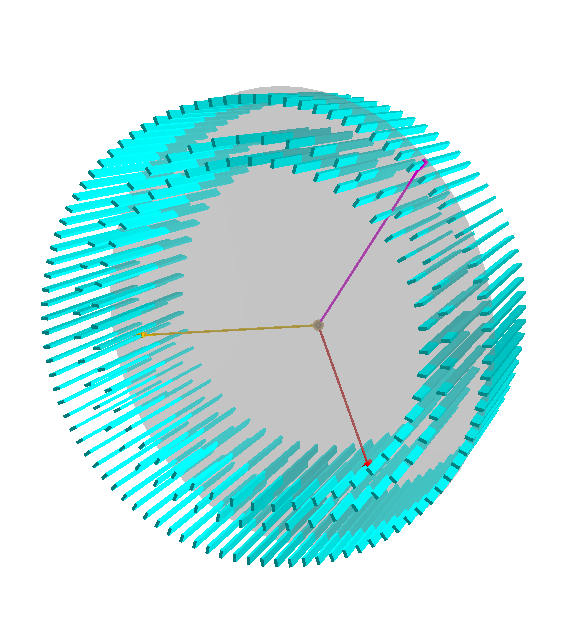
\includegraphics[width=0.4\textwidth]{Chapter6_gps/img/trilateration_jpet_3d}}
  \sidecaption{The reconstruction problem from (A) is transformed to a 2-dimensional problem contained in the decay plane. In this plane, the recording point of each photon is characterized by 2 Cartesian coordinates $X'_i$ and $Y'_i$ (where prime denotes 3D coordinates transformed to the decay plane) and recording time $T_i$}{subfig:b}
  \raisebox{-0.7\height}{\hspace{1cm}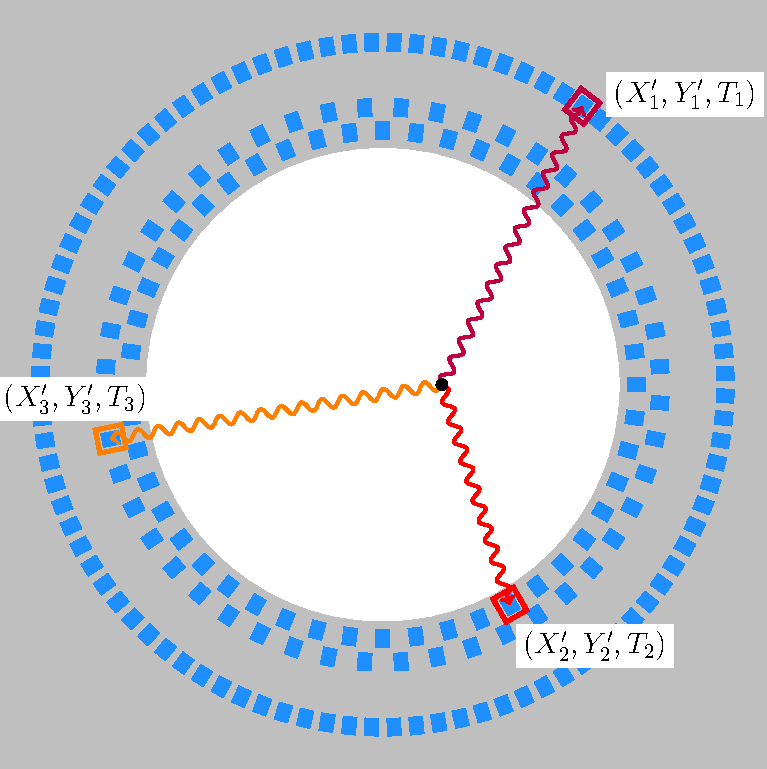
\includegraphics[width=0.4\textwidth]{Chapter6_gps/img/trilateration_jpet_1}}
  \sidecaption{For each of the three recorded photon interactions, a set of possible photon creation points, which would allow for its interaction in time $T_i$ at the position $X'_i,Y'_i$, is constituted by a circle centered at $X'_i,Y'_i$ with a variable radius given by $R_i(t)=c(T_i-t)$ where $t$ is an unknown time of the o-Ps annihilation. The annihilation point $(x',y')$, being a common origin of the three photons, can be found as an intersection of such three circles. \ops/ annihilation time $t$ is obtained as a by-product of the reconstruction.}{subfig:c}
  \raisebox{-0.9\height}{\hspace{1cm}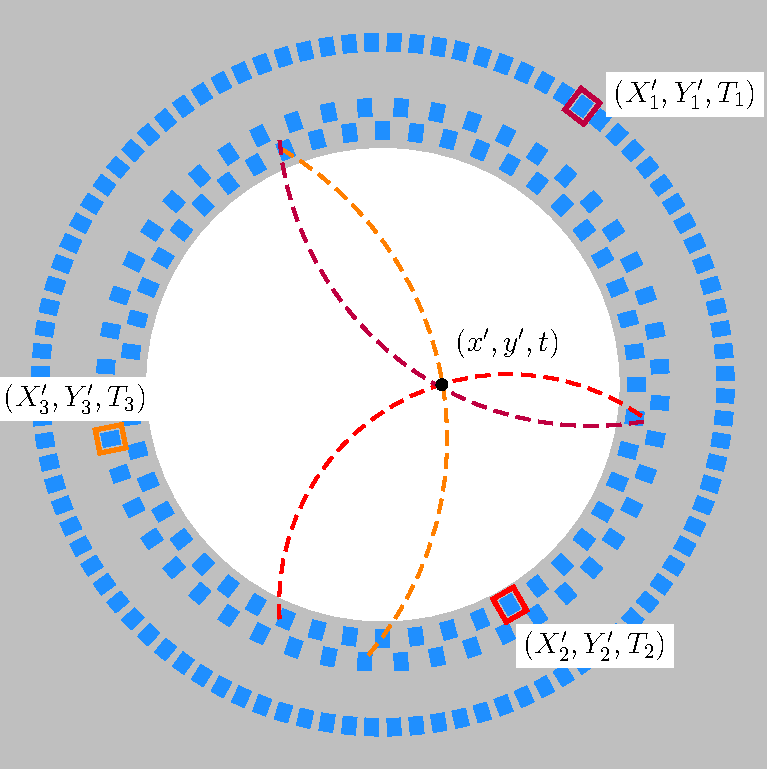
\includegraphics[width=0.4\textwidth]{Chapter6_gps/img/trilateration_jpet_2}}
  \caption{Scheme of o-Ps$\to 3 \gamma$ decay reconstruction in J-PET.}\label{fig:trilateration_jpet}
\end{figure}

For each of the recorded photon interaction points, its spatial coordinates and time $(\!X_i,\!Y_i,\!Z_i,\!T_i\!)$ are determined as described in~\sref{sec:jpet}. If their locations are expressed with pointing vectors $\vec{r}_1,\vec{r}_2,\vec{r}_3$ with respect to origin of the \jpet/ coordinate system (\fref{fig:jpet_detector}, left), a normal to the decay plane is given by:
\begin{equation}
  \label{eq:jpet_rec_normal}
  \hat{n} = \frac{(\vec{r}_2 - \vec{r}_1) \times (\vec{r}_3 - \vec{r}_1)}{\abs{(\vec{r}_2 - \vec{r}_1) \times (\vec{r}_3 - \vec{r}_1)}}. 
\end{equation}
Before vertex reconstruction, the pointing vectors of $\gamma$ recording points are transformed in the following way:
\begin{equation}
  \label{eq:jpet_gps_transformation}
  \vec{r_i}' \equiv (X'_i,Y'_i,0)  = \mathbf{T}(\vec{v})\mathbf{R}(\angle (\hat{n},\hat{z}),\;\hat{n}\times\hat{z}) \vec{r}_i, \quad i=1,2,3,
\end{equation}
where $\hat{z}$ is the $z$ axis of the detector frame of reference, $\mathbf{R}(\alpha, \hat{k})$ denotes a rotation by an angle $\alpha$ around a $\hat{k}$ axis and $\mathbf{T}(\vec{v})$ is a translation by a vector required to set the decay plane after rotation to $z=0$ in the detector frame. As a result, the problem is reduced to a 2-dimensional space where for each $\gamma$ interaction point in the detector, the set of potential creation points of the photon is constituted by a circle centered in that point and with a radius parametrized by an unknown time of \ops/ decay $t$:
\begin{equation}
  \label{eq:jpet_gps_circles}
  (X'_i-x)^2 + (Y'_i-y)^2 = c^2(T_i-t)^2, \quad i=1,2,3.
\end{equation}

The \ops/$\to 3\gamma$ annihilation point can again be found as a common origin point of all three photons in an event, i.e.\ at an intersection of the variable-radius spheres shown in~\fref{subfig:c}. Similarly as in the 3-dimensional case, to solve such a system one more reference point is needed with respect to the problem of intersecting fixed-radii circles, so that all three photons must be detected to enable event reconstruction. The annihilation point on the decay plane $(x',y',0)$ is found analytically as a solution of the above equation system, which also yields the time $t$ of the decay alike the $\Kl\to 3\pi^0$ reconstruction. A comprehensive recipe for an analytical solution of the system from~\eref{eq:jpet_gps_circles} is presented in~\aref{appendix:jpet_solution}. %As shown therein, the decay point and time may be determined with a two-fold ambiguity. In such cases, additional criteria must be used to distinguish the physical solution from a reconstruction artifact.

The final reconstruction step comprises transformation of the solution from the decay plane back to the 3-dimensional frame of reference of the detector:
\begin{equation}
  \label{eq:jpet_gps_transformation_inverse}
  (x,y,z) = \mathbf{R}(-\angle (\hat{n},\hat{z}),\;\hat{n}\times\hat{z}) \mathbf{T}(-\vec{v}) (x',y',0).
\end{equation}

The reconstruction method presented above has been comprehensively tested with MC simulations in order to assess its resolution and applicability for the studies described in~\cref{chapter:test_jpet}~\cite{gajos_gps}. Moreover, its employment in a novel medical imaging technique is the subject of a patent application~\cite{imaging_patent}. Preliminary tests with the first recorded sample of annihilations into three photons have also been performed and their results are presented in~\cref{chapter:analysis_jpet}.

%%% Local Variables:
%%% TeX-master: "../main"
%%% End: